%Dokument til projektafgrænsningen
\subsection{Projektafgrænsning}

Vi har planlagt at arbejde med en kanon som skal kunne rotere 360 grader, samt have et vinkelinterval til affyring af kanonen på mindst 100 grader. Den fjernstyrede kanon skal være i stand til at modtage information fra et kontrolmodul. Dette skal ske ved brug af en bluetooth enhed eller et andet trådløst kommunikationsmodul. Der skal altså laves en mikrocontroller som kan styre kanonen gennem disse trådløse moduler ved at få kommandoer fra et kontrolmodul.\\

\begin{figure}[H]
\centering
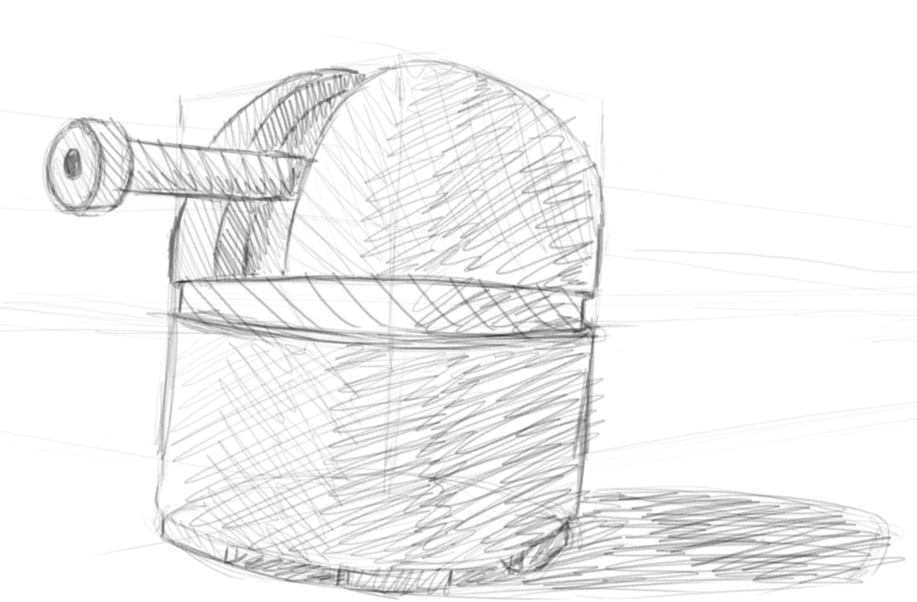
\includegraphics[scale=0.4]{Billeder/Koncept_turret.png}
\caption{Koncept af kanon.}
\label{fig:KonceptKanon}
\end{figure}

Selve kanons affyringsmekanisme er en pneumatisk gearkasse, der trækker en fjeder op, som derefter affyrer skuddet. Vi modificerer dog mekanismen, så man ikke længere skal bruge aftrækkeren, men istedet kan styre affyringen med en knap, hvis signal bliver sendt trådløst. Selve kanonens krop laves vha. 3D print af de enkelte komponenter, der sættes sammen med enten lim eller skruer. \\

Til udarbejdningen af det fysikvidenskabelige dokumentation kan der påmonteres forskellige accelerometerer, som kan bruges til at bestemme skydevinklen. Derudover kan der alternativt måles, hvor langt projektilet bliver affyret for så, at kunne beregne dets hastighed, hvis affyringsvinklen er kendt.

\begin{figure}[H]
\centering
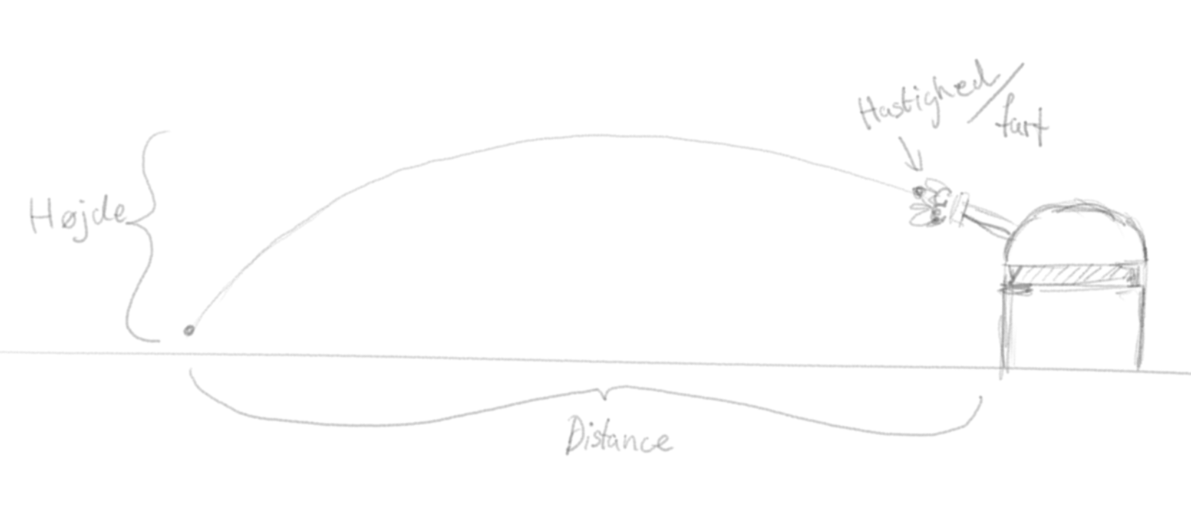
\includegraphics[scale=0.4]{Billeder/Fysik_koncept.png}
\caption{Fysik relevant til kanonen.}
\label{fig:FysikKoncept}
\end{figure}